\begin{frame}{Commutative Diagram}
\begin{center}
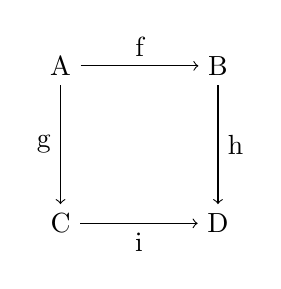
\begin{tikzpicture}[node distance=2cm]
    \node (A) {A};
    \node[right of=A] (B) {B};
    \node[below of=A] (C) {C};
    \node[below of=B] (D) {D};
    
    \draw[->] (A) -- node[above] {f} (B);
    \draw[->] (A) -- node[left] {g} (C);
    \draw[->] (B) -- node[right] {h} (D);
    \draw[->] (C) -- node[below] {i} (D);
\end{tikzpicture}
\end{center}

\footnotesize
\texttt{\textbackslash draw[->] (A) -- node[above] \{f\} (B);}
\end{frame}